\documentclass{statsmsc}
\usepackage{float}
\usepackage{hyperref}
\usepackage[utf8]{inputenc}
\usepackage{graphicx}
\usepackage{caption}
\usepackage{subcaption}
\usepackage{algpseudocode}
\usepackage{algorithm}
\usepackage{mathtools}
\usepackage{amsmath,amssymb}
\usepackage{nccmath}
\usepackage{siunitx}
\usepackage{listings}
\usepackage{physics}
\usepackage{tikz}
\usepackage[outline]{contour} % glow around text
\usepackage{bbm}
\usepackage[most]{tcolorbox}
\newcommand{\e}[1]{{\mathbb E}\left[ #1 \right]}
\definecolor{block-gray}{gray}{0.90}
\newtcolorbox{code}{colback=block-gray,grow to right by=-1mm,grow to left by=-1mm,boxrule=0pt,boxsep=0pt,breakable}
\lstset{
  basicstyle=\ttfamily,
  columns=fullflexible,
  frame=single,
  breaklines=true,
  postbreak=\mbox{\textcolor{red}{$\hookrightarrow$}\space},
}
\usetikzlibrary{patterns,snakes}
\usetikzlibrary{arrows.meta} % for arrow size
\contourlength{0.4pt}

\colorlet{xcol}{blue!70!black}
\colorlet{darkblue}{blue!40!black}
\colorlet{myred}{red!65!black}
\tikzstyle{mydashed}=[xcol,dashed,line width=0.25,dash pattern=on 2.2pt off 2.2pt]
\tikzstyle{axis}=[->,thick] %line width=0.6
\tikzstyle{ell}=[{Latex[length=3.3,width=2.2]}-{Latex[length=3.3,width=2.2]},line width=0.3]
\tikzstyle{dx}=[-{Latex[length=3.3,width=2.2]},darkblue,line width=0.3]
\tikzstyle{ground}=[preaction={fill,top color=black!10,bottom color=black!5,shading angle=20},
                    fill,pattern=north east lines,draw=none,minimum width=0.3,minimum height=0.6]
\tikzstyle{mass}=[line width=0.6,red!30!black,fill=red!40!black!10,rounded corners=1,
                  top color=red!40!black!20,bottom color=red!40!black!10,shading angle=20]
\tikzstyle{spring}=[line width=0.8,blue!7!black!80,snake=coil,segment amplitude=5,segment length=5,line cap=round]
\tikzset{>=latex} % for LaTeX arrow head
\tikzstyle{force}=[->,myred,very thick,line cap=round]
\def\tick#1#2{\draw[thick] (#1)++(#2:0.1) --++ (#2-180:0.2)}
\newsavebox{\overlongequation}
\newenvironment{CentreLongEquation}
 {\begin{displaymath}\begin{lrbox}{\overlongequation}$\displaystyle}
 {$\end{lrbox}\makebox[0pt]{\usebox{\overlongequation}}\end{displaymath}}


\title{Learning Invariances in Dynamical System}
\author{Cheng-Cheng Lao}
\CID{01353756}
\supervisor{Dr. Andrew Duncan and Dr. Mark van der Wilk}
\date{\today}
%For today's date, use:
%\date{\today}
\logoimg{}


% THIS IS WHERE NEW COMMANDS CAN BE DEFINED
% commands below only used in the proof; otherwise can be deleted
\newcommand{\consta}{a}
\newcommand{\X}{X}
\newcommand{\EE}[1]{ \mathrm{E} [ #1 ] }
\newcommand{\inparenth}[1]{\left( #1 \right)}

\begin{document}

% Generates the Title Page
\maketitle


% Generates plagiarism declaration
\declarationname{Cheng-Cheng Lao}
\declarationdate{\today}
\declaration 


\begin{abstract}
    ABSTRACT GOES HERE
\end{abstract}

\begin{acknowledgements}
    ANY ACKNOWLEDGEMENTS GO HERE
\end{acknowledgements}

% add glossary?

% VERY IMPORTANT
% This command switches from Roman to Arabic numbering for main part of thesis
\mainmatter


\chapter{Introduction}

The introduction section goes here\footnote{Tip: write this section last.}.

\chapter{Background}
Here we will cover the background knowledge required to understand the remaining thesis, including theortical foundation of Gaussian Process, dynamical systems and invariances. 

Background chapter.

\section{Gaussian Process}
Gaussian Process (GP)

Section content goes here. 

\subsection{My subsection}

A subsection.

\subsubsection{My subsubsection}

A subsubsection.
\section{Dynamical Systems}
A dynamical system is simply a system that evolves with time under some kind of rules.
\section{Invariances}
Invariances are functions of the states that describe a dynamical system, and is unchanged throughout the evolution of the system over time. 
An example would be from the field of physics, the conservation of energy, which will be unchanged throught out the trajectories of the system.

\section{Figures}

It is better to create figures in a vector-based format, such as PDF.

\begin{figure}[!h]
    \centering
    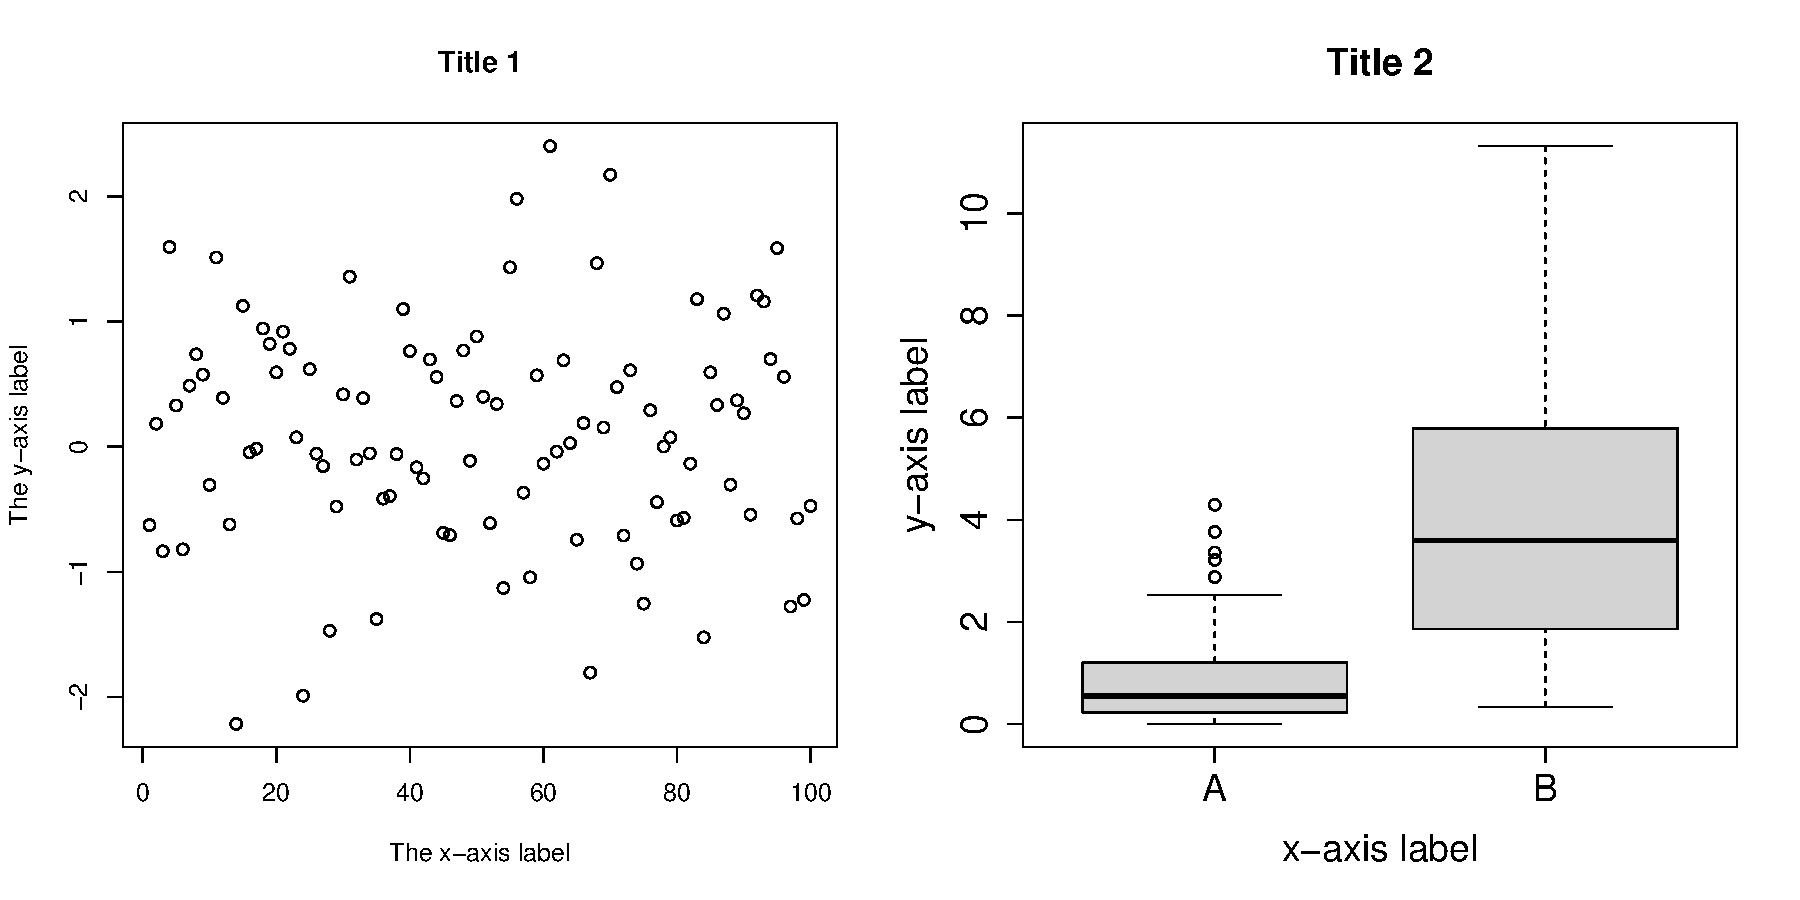
\includegraphics[width=\textwidth]{fig1.pdf}
    \caption{Remember to make fonts in figures large enough (compare the two figures.)}
    \label{fig:fig1}
\end{figure}

\section{Tables}

\label{sec:tablesection}

Here is an example of a table

\begin{table}[ht]
\centering
\begin{tabular}{rr}
  \hline
    $z$& $\textrm{P}(Z < z)$ \\
  \hline
    1.281& 0.900\\
    1.645& 0.950\\
    1.960& 0.975\\
    2.326& 0.990 \\
    2.576& 0.995 \\
   \hline
\end{tabular}
    \caption{Partial table showing values of $z$ for $\textrm{P}(Z < z)$, 
    where $Z$ has a standard normal distribution.}
    \label{tab:normal}
\end{table}



\section{Referencing sources, sections and items}

A good book on the bootstrap is \cite{efrontib}, although the idea
appeared in an earlier paper \citep{efron1979}.

Note that to make the references appear, you will need to compile
the bibtex, otherwise you may just see question marks where the references
should be.


\subsection{Referencing sections, results and equations}

Theorem~\ref{thm:theorem1} is proved in Section~\ref{sec:defnthms}; see 
Equation~\eqref{eqn:second}.



\subsubsection{Referencing tables and figures}

When labelling figures and tables, it is important that the label command
\texttt{\textbackslash label\{LABELNAME\}} comes \textbf{after} the caption command.
See Table~\ref{tab:normal} and Figure~\ref{fig:fig1} above.

\subsection{Quoting sources}
If you wish to quote a source, be sure to use quotation marks and cite the
reference. The \texttt{\textbackslash{usequote}} command is useful here:

\usequote{It was the best of times, it was the worst of times, it was the age of wisdom, it was the age of foolishness, it was the epoch of belief, it was the epoch of incredulity, it was the season of Light, it was the season of Darkness, it was the spring of hope, it was the winter of despair, we had everything before us, we had nothing before us, we were all going direct to Heaven, we were all going direct the other way - in short, the period was so far like the present period, that some of its noisiest authorities insisted on its being received, for good or for evil, in the superlative degree of comparison only.} \citep{dickens1859}

% forcing a page break
\clearpage


\section{Definitions, theorems and examples}
\label{sec:defnthms}

The following environments are supported:
Definition, Theorem, Proof, Proposition, Lemma, Remark, Example.

\begin{definition}
    The \textbf{variance} of a random variable $X$ is defined as
    \begin{equation}
        \mathrm{Var}(X) = \mathrm{E}[(X - \mathrm{E}[X])^2].
    \end{equation}
\end{definition}

\begin{theorem}
    \label{thm:theorem1}
Given a random variable $X$, over all values $a \in \mathbb{R}$, 
\begin{equation}
    \min_{a \in \mathbb{R}} \mathrm{E}[(X - a)^2] 
    = \mathrm{E}[(X - \mathrm{E}[X])^2].
    \label{eqn:second}
\end{equation}
\end{theorem}

\begin{proof}   
    Starting with the left-hand side,
\begin{align}
% Example of using \newcommands; see above
\EE{ \inparenth{\X - \consta}^2 } 
&=  \EE{  \inparenth{\X - \EE{\X} + \EE{\X} - \consta}^2 } 
    \nonumber \\
&=  \EE{  \inparenth{ \X - \EE{\X} }^2 } 
    + 2 \EE{ \inparenth{ \X - \EE{\X} } \inparenth{ \EE{\X} - \consta} } +  
  \EE{ \inparenth{ \EE{\X} - \consta}^2  }    
    \nonumber \\
&=  \EE{  \inparenth{ \X - \EE{\X} }^2 } +  \inparenth{ \EE{\X} - \consta}^2
    \nonumber \\
& \geq \EE{  \inparenth{ \X - \EE{\X} }^2 },  
\nonumber 
\end{align}
since $\EE{\X}$ is a real number and $\inparenth{ \EE{\X} - \consta}^2 \geq 0$,
and the third line follows from linearity of expectation:
\begin{align}
    \EE{ \inparenth{ \X - \EE{\X} } \inparenth{ \EE{\X} - \consta} }
    =
    \inparenth{ \EE{\X} - \consta} \EE{ \inparenth{ \X - \EE{\X} } }
    =
    \inparenth{ \EE{\X} - \consta}  \inparenth{\EE{ \X} - \EE{\X} } 
    =
    0,
    \nonumber
\end{align}
    since $\EE{\EE{\X}} = \EE{\X}$, which proves the result.
\end{proof}

\begin{remark}
    This theorem shows that that the minimum of the quantity
    $\mathrm{E}[(X - a)^2]$ is equal to $\mathrm{Var}(X)$.
    In some sense, this makes the variance a natural measure of dispersion if 
    we are taking the metric to be the squared deviation of $X$.
\end{remark}


\begin{lemma}[Stein's Lemma]
    Let $X \sim \mathrm{N}(\mu, \sigma^2)$, and let $g$ be a differentiable 
    function satisfying $\mathrm{E}[|g'(X)|] < \infty$. Then
    \begin{equation}
        \mathrm{E}[g(X)(X-\mu)] = \sigma^2 \mathrm{E}[g'(X)].
        \nonumber
    \end{equation}
\end{lemma}

\begin{proposition}[Popoviciu's inequality]
    Suppose that the random variable $X$ is known to only take values in the 
    bounded range $[a, b]$. Then  
    \begin{align}
        \mathrm{Var}[X] \leq \dfrac{(b-a)^2}{4}.
        \nonumber
    \end{align}
\end{proposition}

\begin{example}
    Suppose $X \sim \mathrm{Bern} (p)$, for some $p \in [0,1]$. Then, 
    since $X \in \{0, 1\}$, $X$ is bounded between $0$ and $1$ and so
    $\mathrm{Var}[X] \leq \tfrac{1}{4}$.
\end{example}

\chapter{Invariance Kernel}
In this chapter we will start with general theoretical construction of invariance kernel given the knowlwedge of the invariance of the system.
We will then apply the construction to various systems, namely linear and nonlinear system in both one and two dimensions.
\section{General Construction}
If we are given a dynamical system of dimension d with variables $\mathbf{q}, \mathbf{p}$, where $\mathbf{q} = (q_1, q_2,\dots,q_d)$ is the vector of positional coordinates, and $\mathbf{p}=(p_1, p_2, \dots, p_d)$ is the vector of velocity coordinates of the states of the dynamical system.
We are interested to predict the future trajectories of the state of the system.
Therefore, we would like to know the time derivative of these coordinates so we can update them according to Euler's integrator. 
These time derivatives are referred to as the dynamics of a dynamical system, which governs the evolution of the dynamical system, and is a function of the coordinates $\mathbf{q}$ and $\mathbf{p}$ 
For our systems, we will denote the dynamics of $\mathbf{p}$ as $\frac{d\mathbf{p}}{dt}=\mathbf{a}(\mathbf{q}, \mathbf{p})$, and that of $\mathbf{q}$ as $\frac{d\mathbf{q}}{dt}=\mathbf{v}(\mathbf{q}, \mathbf{p})$.
Once we have the dynamics, we can integrate up to obtain the future trajectories. 
Notation wise, we will collect the two dynamics term and call them $$\mathbf{f(\mathbf{q}, \mathbf{p})}=\begin{pmatrix}
    \mathbf{a(\mathbf{q}, \mathbf{p})}\\\mathbf{v(\mathbf{q}, \mathbf{p})}
\end{pmatrix}$$
For simplicity of notation, the dependence on $\mathbf{q}, \mathbf{p}$ is now implicit. 
We will put independent GP prior on $\mathbf{a}$ and $\mathbf{v}$ since there are no reason we should assume they are correlated. 
For the choice of kernel, we chose the standard smooth kernel, the squared exponential kernel, or RBF, and we denote this kernel to be $K_{RBF}$. 
We will also denote any set of coordinates of length $n$ and dimension $d$ as $$X=\begin{pmatrix}
    q_{11}& q_{21} &\dots& q_{d1} & p_{11} & p_{21} & \dots & p_{d1} \\
    q_{12}& q_{22} &\dots& q_{d2} & p_{12} & p_{22} & \dots & p_{d2} \\
    \vdots &\vdots &\ddots &\vdots &\vdots &\vdots &\ddots &\vdots \\
    q_{1n}& q_{2n} &\dots& q_{dn} & p_{1n} & p_{2n} & \dots & p_{dn} \\
\end{pmatrix}=\begin{pmatrix}
    \mathbf{x}_1\\\mathbf{x}_2\\\vdots\\\mathbf{x}_n
\end{pmatrix}.$$
Without loss of generality, we will choose to stack the dynamics vertically in $\mathbf{f}$; for example in a d dimensional system, we have $$\mathbf{f}(X)=\begin{pmatrix}
    a_1(\mathbf{x}_1)\\
    \vdots\\
    a_1(\mathbf{x}_n)\\
    a_2(\mathbf{x}_1)\\
    \vdots\\
    a_2(\mathbf{x}_n)\\
    \vdots\\
    a_d(\mathbf{x}_1)\\
    \vdots\\
    a_d(\mathbf{x}_n)\\
    v_1(\mathbf{x}_1)\\
    \vdots\\
    v_1(\mathbf{x}_n)\\
    v_2(\mathbf{x}_1)\\
    \vdots\\
    v_2(\mathbf{x}_n)\\
    \vdots\\
    v_d(\mathbf{x}_1)\\
    \vdots\\
    v_d(\mathbf{x}_n)\\
\end{pmatrix}$$
For our naive independent RBF GP prior, we have 
\begin{CentreLongEquation}
$$
K=\mathrm{Cov}(\mathbf{f}(X), \mathbf{f}(X'))=\begin{pmatrix}
    K_{RBF,a_1}(X,X') & \dots  & \dots          & \dots         & 0\\
    \vdots        & \ddots & \dots          & \ddots        & \vdots\\
    0             & \dots  & K_{RBF,a_d}(X,X')  & \dots         & 0 \\
    \vdots        & \ddots & \vdots         & K_{RBF,v_1}(X,X') & \vdots \\
    0             & \dots  & 0              & \dots         & K_{RBF,v_d}(X,X')\\
\end{pmatrix},
$$
\end{CentreLongEquation}

with all the off diagonal terms being zero block matrix because of the independence prior assumption.
This naive kernel will be our baseline to be compared to throughout the whole project.
Now we can start considering the invariance. 
If we assume the invariance is true throughout the input space $\mathbb{R}^{2d}$, then we can condition the GP on the a grid of points, which we referred to invariance points, $X_L$, and assume it has length $\ell$, and we will call the invariance constraints $L$.
The form of $L$ will depend on the system as well as $X_L$, and examples will be described in the following sections.
Since the invariance function will always be a linear function on the dynamics, if we apply this linear transformation $L$ on $\mathbf{f}(X_L)$, $L(\mathbf{f}(X_L))$ will again be a GP with a transformed kernel.
Therefore, we have 
$$\begin{pmatrix}
\mathbf{f}(X)\\L[\mathbf{f}(X_L)]
\end{pmatrix}
\sim\mathcal{N}
\left(\begin{pmatrix}0_{2nd}\\0_{\ell}\end{pmatrix}, \begin{pmatrix}
    K & LK \\
    KL^T & LKL^T\\
\end{pmatrix}\right)
$$

\section{1D System}
\subsection{Linear}
We will first examine one of the most simple dynamical system, an 1D simple harmonic motion (SHM). 
An example would be a mass spring system as shown in figure with mass $m$ and spring constant $k$. 

% HORIZONTAL spring - axis, rest position
\begin{figure}[H]
    \centering
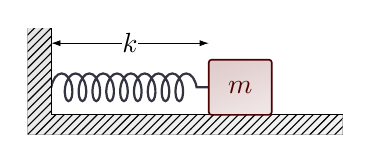
\begin{tikzpicture}
  \def\H{1.1}  % wall height
  \def\T{0.3}  % wall thickness
  \def\W{3.7}  % ground length
  \def\D{0.25} % ground depth
  \def\h{0.7}  % mass height
  \def\w{0.8}  % mass width
  \def\x{2.0}  % mass x position
  \def\y{1.22*\H} % x axis y position
  
  % AXIS
  \draw[ell] (0,1.3*\h) --++ (\x,0) node[midway,fill=white,inner sep=0] {$k$};
  
  % SPRING & MASS
  \draw[spring] (0,\h/2) --++ (\x,0);
  \draw[ground] (0,0) |-++ (-\T,\H) |-++ (\T+\W,-\H-\D) -- (\W,0) -- cycle;
  \draw (0,\H) -- (0,0) -- (\W,0);
  \draw[mass] (\x,0) rectangle++ (\w,\h) node[midway] {$m$};
  
\end{tikzpicture}
\end{figure}

The defining equation is $$m\frac{d^2q}{dt^2}=-kq$$, where $q$ is the displacement.
And the analytical solution would be of the form $q=A\sin(\omega_0t+\phi),$ where $\omega=\frac{k}{m}$ and $A, \phi$ depends on the initial condition, which dictates the amplitude and phase of the motion. 
For this case, we have 
$$
\mathbf{f}(X)=\begin{pmatrix}
    \mathbf{a}(X)\\
    \mathbf{v}(X)\\
\end{pmatrix}
$$
We also have the energy, $E=\frac{kq^2}{2}+\frac{mp^2}{2},$
Therefore, to obtain our invariance $L$, we use the conservation of energy $\frac{dE}{dt}=0$ so we finally have $$L(a, v)=kqv+mpa=0$$
In our system, since the only parameters that control the periodicity of the oscillation is $k$ and $m$, but they only come in as the ratio between them. 
For simplicity, I will assume $k=m=1$ so $\omega_0=1.$ 
While $L$ is not able to be into a matrix form, it is an linear operator as shown below. 
If we have $$X_L=\begin{pmatrix}
    q_{L,1} & p_{L,1}\\
    \vdots & \vdots \\
    q_{L,\ell} & p_{L,\ell}\\
\end{pmatrix}=\begin{pmatrix}
    \vdots & \vdots\\
    q_L & p_L\\
    \vdots & \vdots\\
\end{pmatrix}=\begin{pmatrix}
    \mathbf{x}_{L,1}\\
    \vdots\\
    \mathbf{x}_{L,\ell}\\
\end{pmatrix},$$
then we have 
$$
L([\mathbf{f}(X_L)]) = \begin{pmatrix}
   p_{L,1}a(q_{L,1},p_{L,1}) + q_{L,1}v(q_{L,1},p_{L,1})\\ 
   \vdots \\
   p_{L,\ell}a(q_{L,\ell},p_{L,\ell}) + q_{L,\ell}v(q_{L,\ell},p_{L,\ell})\\ 
\end{pmatrix}.
$$
Combine with original GP prior assumption, we will have 
$$
\begin{pmatrix}
    \mathbf{f}(X)\\
    L([\mathbf{f}(X_L)])\\
\end{pmatrix}
\sim\mathcal{N}
\left(\begin{pmatrix}
    0_{2nd}\\0_{\ell}
\end{pmatrix},\begin{pmatrix}
   A & B \\
   C & D\\ 
\end{pmatrix}\right),
$$
where
$$
A=K(X,X), B=\begin{pmatrix}
    K_{RBF,a} \\ K_{RBF,v} \\
\end{pmatrix}\odot \begin{pmatrix}
    P_L \\ Q_L
\end{pmatrix}, C=B^T, D=K_{RBF,a}\odot (p_L\otimes p_L) + K_{RBF,v}\odot (q_L\otimes q_L),
$$
where $\odot$ is the element wise product and $\otimes$ is the Kronecker product so that 
$$
P_L=\begin{pmatrix}
  p_{L,1}  & \dots & p_{L,\ell}  \\
  \vdots & \text{repeats n rows} &  \vdots\\
  p_{L,1}  & \dots & p_{L,\ell}  \\
\end{pmatrix},
Q_L=\begin{pmatrix}
  q_{L,1}  & \dots & q_{L,\ell}  \\
  \vdots & \text{reqeats n rows} &  \vdots\\
  q_{L,1}  & \dots & q_{L,\ell}  \\
\end{pmatrix}
$$
and we have 
$$
p_L\otimes p_L=\begin{pmatrix}
  p_{L,1}^2 & p_{L,1}p_{L,2} & \dots & p_{L,1}p_{L,\ell} \\
  \vdots & \vdots & \vdots & \vdots \\
  p_{L,\ell}p_{L,1} & p_{L,\ell}p_{L,2} & \dots & p_{L,\ell}^2 \\
\end{pmatrix},
q_L\otimes q_L=\begin{pmatrix}
  q_{L,1}^2 & q_{L,1}q_{L,2} & \dots & q_{L,1}q_{L,\ell} \\
  \vdots & \vdots & \vdots & \vdots \\
  q_{L,\ell}q_{L,1} & q_{L,\ell}q_{L,2} & \dots & q_{L,\ell}^2 \\
\end{pmatrix},
$$ 
These matrices can be obtained if we try to compute the covariance manually. 
For $B$, we wish to calculate 

\begin{align*}
B_{ij} &= \mathrm{Cov}(\mathbf{f}(X), L[\mathbf{f}(X_L)])_{ij} \\
       &= \mathrm{Cov}(\mathbf{f}(X)_i, L\mathbf{f}(X_L)_j) \\ 
       &= \begin{cases}
        \mathrm{Cov}(a(q_i, p_i), p_{L,j}a(q_{L,j},p_{L,j}) + q_{L,j}v(q_{L,j},p_{L,j})) & i\le n \\ 
        \mathrm{Cov}(v(q_i, p_i), p_{L,j}a(q_{L,j},p_{L,j}) + q_{L,j}v(q_{L,j},p_{L,j})) & i>n \\ 
       \end{cases} \\
       &= \begin{cases}
        K_{RBF,a}(\mathbf{x}_i, \mathbf{x}_{L,j}) p_{L,j} & i\le n \\ 
        K_{RBF,v}(\mathbf{x}_i, \mathbf{x}_{L,j}) q_{L,j} & i>n \\ 
       \end{cases}, \\
\end{align*}
and hence we have the form above. 
For $D$, we have
\begin{align*}
D_{ij} &= \mathrm{Cov}(L[\mathbf{f}(X_L)], L[\mathbf{f}(X_L)])_{ij} \\
       &= \mathrm{Cov}(p_{L,i}a(q_{L,i},p_{L,i}) + q_{L,i}v(q_{L,i},p_{L,i}), p_{L,i}a(q_{L,i},p_{L,i}) + q_{L,i}v(q_{L,i},p_{L,i})) \\
       &= p_{L,i}p_{L,j}K_{RBF,a}(\mathbf{x}_{L,i},\mathbf{x}_{L,j}) + q_{L,i}q_{L,j}K_{RBF,v}(\mathbf{x}_{L,i},\mathbf{x}_{L,j})
\end{align*}
using the bilnear property of the covariance operator and the fact that $v$ and $a$ are independent.
Since we assume invariance on these invariance points, we will condition on $L([\mathbf{f}(X_L)])=0.$
Now we can simply use the Gaussian conditional formula to obtain the Schur Complement
$$
\mathbf{f}(X)|L[\mathbf{f}(X_L)]=0\sim\mathcal{N}(0_{2n},A-BD^{-1}C),
$$
we will then call the covariance part our Invariance Kernel for 1D SHM, $K_L$.
\subsection{Non Linear}
The story is pretty much the same for nonlinear system, it is just the fitting would be expected to be more difficult.
A simple nonlinear system in every day life is a simple pendulum as shown in figure below.
The governing equation is 
$$
\frac{d^2q}{dt^2}=-\frac{g}{\ell}\sin q, 
$$
where $q$ is the angle of displacement this time. 
The nonlinear dynamics bit occurs because of the sine term, which will complicate things slightly. 
However, since $\sin x \approx x$ at small angle, this system is approximately linear under small displacement. 
For simplicity, I will again set $g=\ell=1$.
There is no analytical solution to this nonlinear problem.
This time we have energy, $E=\frac{m\ell^2p^2}{2}+mg\ell(1-\cos q)$, and by setting the time derivative to 0, we have $$L(a, v)=\frac{dE}{dt}=m\ell^2pa+mg\ell\sin qv=0.$$
If we cancel out the common term $m\ell$ since their product cannot be zero, we have $$L(a,v)=\ell pa+g\sin qv=0$$
Most of the terms are unchanged from the linear case. 
However, this time, 
$$
B=\begin{pmatrix}
    K_{RBF,a} \\ K_{RBF,v} \\
\end{pmatrix}\odot \begin{pmatrix}
    P_L \\ \sin(Q_L)
\end{pmatrix}, D=K_{RBF,a}\odot (p_L\otimes p_L) + K_{RBF,v}\odot (\sin(q_L)\otimes \sin(q_L)),
$$
where 
$$
\sin(Q_L) = \begin{pmatrix}
  \sin(q_{L,1})  & \dots & \sin(q_{L,\ell})  \\
  \vdots & \text{reqeats n rows} &  \vdots\\
  \sin(q_{L,1})  & \dots & \sin(q_{L,\ell})  \\
\end{pmatrix},
$$
$$
\sin(q_L)\otimes \sin(q_L)=\begin{pmatrix}
  \sin(q_{L,1})^2 & \sin(q_{L,1})\sin(q_{L,2}) & \dots & \sin(q_{L,1})\sin(q_{L,\ell}) \\
  \vdots & \vdots & \vdots & \vdots \\
  \sin(q_{L,\ell})\sin(q_{L,1}) & \sin(q_{L,\ell})\sin(q_{L,2}) & \dots & \sin(q_{L,\ell})^2 \\
\end{pmatrix},
$$
derived in almost exactly the same way as the linear case. 
\section{Damped System}
Before we have considered a perfect system, i.e. a system in an ideal world without frictions and the conservation of energy is perfectly obeyed such that $L=0$ exactly.
However, in a real world system, there will be dissipation where energy is lost in the form of heat etc.  
Therefore, to model that, we need to allow "approximate" invariance, such that the invariance $L$ is noisy and not always equal to zero. 
To do so, it is similar in spirit to when we add noise to the underlying GP to represent noise signal, where we have $K+\sigma_n^2 \mathbb{1}$.
Here, since the white noise is uncorrelated, the only place the noise will enter is $D$, so we simply have to add a noise term to $D$ and replace all $D$ with $\tilde{D}=D+\epsilon \mathbb{1}$, where $\epsilon$ is a parameter to be learnt. 
\section{2D System}
A 2D system is not that different from an 1D system. The major difference being there are two more extra variables. 
We again look at two simple examples, a linear 2D SHM, and a nonlinear double pendulum.
\subsection{Linear}
A simple extension to 1D SHM to 2D is just allowing the spring to be at an angle so that the system is now in a 2D space.
Again, the equations are simple that we have two equations for the two coordinates.
$$
\begin{cases}
    \frac{d^2{q_1}}{dt^2} = -\frac{k}{m}q_1\\
    \frac{d^2{q_2}}{dt^2} = -\frac{k}{m}q_2\\
\end{cases}
$$
The analytical solution is exactly the same, but now there are two of them with differing amplitudes and phases depending on the initial condition. 
And now we have $$\mathbf{f}(X)=\begin{pmatrix}
    \mathbf{a_1}(X)\\
    \mathbf{a_2}(X)\\
    \mathbf{v_1}(X)\\
    \mathbf{v_2}(X)\\
\end{pmatrix},$$
where $\mathbf{a_1}$ and $\mathbf{a_2}$ are the dynamics or time derivative for $\mathbf{p_1}$ and $\mathbf{p_2}$ respectively; similarly $\mathbf{v_1}$ and $\mathbf{v_2}$ are the time derivative of $\mathbf{q_1}$ and $\mathbf{q_2}$.
In this system, the energy is the sum of energy in the two directions so $E=\frac{m(p_1^2+p_2^2)}{2}+\frac{k(q_1^2+q_2^2)}{2}$ and so the invariance $L(a_1, a_2, v_1, v_2)=mp_1a_1+mp_2a_2+kq_1v_1+kq_2v_2=0.$
Now our naive baseline GP has the kernel
$$
K(X,X')=\begin{pmatrix}
K_{RBF,a_1}(X,X') & 0 & 0 & 0 \\
0 & K_{RBF,a_2}(X,X') & 0 & 0 \\
0 & 0 & K_{RBF,v_1}(X,X') & 0 \\
0 & 0 & 0 & K_{RBF,v_2}(X,X') \\
\end{pmatrix}.
$$
We will then have the joint distribution of
$$
\begin{pmatrix}
    \mathbf{f}(X)\\L[\mathbf{f}(X_L)]\\
\end{pmatrix}
\sim\mathcal{N}
\left(
\begin{pmatrix}
    0_{4n} \\ 0_{\ell}
\end{pmatrix},
\begin{pmatrix}
    A & B \\
    C & D\\
\end{pmatrix}
\right),
$$
with 

\begin{align*}
A&=K(X, X'), 
B=\begin{pmatrix}
    K_{RBF, a_1}\\
    K_{RBF, a_2}\\
    K_{RBF, v_1}\\
    K_{RBF, v_2}\\
\end{pmatrix}\odot
\begin{pmatrix}
P_{1L}  \\
P_{2L}  \\
Q_{1L}  \\
Q_{2L}  \\
\end{pmatrix},
C=B^T,\\ 
D&=K_{RBF,a_1}\odot(p_{1L}\otimes p_{1L}) +K_{RBF,a_2}\odot(p_{2L}\otimes p_{2L})+K_{RBF,v_1}\odot(q_{1L}\otimes q_{1L})+K_{RBF,v_2}\odot(q_{2L}\otimes p_{2L})
\end{align*}
where the terms are defined the exact same way as before, and the derivation are also the same.
We will then again take the Schur Complement.
\subsection{Non Linear}
Now we will to introduce double pendulum, which is a fairly nonlinear system and quite complicated. 
It has two mass blobs $m_1$ and $m_2$ as well as two lengths for the pendlum stem $\ell_1$ and $\ell_2$.
The defining equations are as follows:
$$
\begin{cases}
\frac{d^2q_1}{dt^2}=\frac{-g\left(2 m_{1}+m_{2}\right) \sin q_1-m_{2} g \sin \left(q_1-2 q_2\right)-2 \sin \left(q_1-q_2\right) m_{2}\left(p_2^{2} l_{2}+p_1^{2} l_{1} \cos \left(q_1-q_2\right)\right)}{l_{1}\left(2 m_{1}+m_{2}-m_{2} \cos \left(2 q_1-2 q_2\right)\right)} \\
\frac{d^2q_2}{dt^2}=\frac{2 \sin \left(q_1-q_2\right)\left(p_1^{2} l_{1}\left(m_{1}+m_{2}\right)+g\left(m_{1}+m_{2}\right) \cos q_1+p_2{ }^{2} l_{2} m_{2} \cos \left(q_1-q_2\right)\right)}{l_{2}\left(2 m_{1}+m_{2}-m_{2} \cos \left(2 q_1-2 q_2\right)\right)}
\end{cases}
$$
As we can see, it is very complicated in term of the form.
We also have form of energy 
$$
E = -(m_1+m_2)gl_1\cos q_1-m_2gl_2\cos q_2+ \frac{m_1l^2_1p_1^2}{2}+\frac{m_2}{2}(l^2_1p_1^2+l^2_2p_2^2+2l_1l_2p_1p_2\cos(q_1-q_2))
$$
again for simplicity, we set all constants to unity, so that $m_1=m_2=\ell_1=\ell_2=g=1.$
While the form is more complicated, the underlying principle to construct the invariance kernel. 
\section{Local Invariance}
\chapter{Learning Invariance}
Previously, we have assumed the knowledge of the dynamics equation from Newton's Law, which allowed us to derive the energy and thereafter the invariance equation. 
However, for the kernel to be useful in real life, we cannot assume the equations of the system beforehand, since if we have the knowledge, then the system is pretty much solved that we can just use an ODE integrator to obtain the trajectories. 
Therefore, we should find a way for the system to learn the form of invariance from data directly.
One way to do so is to parameterise our invariance function and allow the system to learn the coefficients by maximising the log marginal likelihood.
\section{1D system}
A simple way to parameterise an unknown function, when the problem is relatively bounded is to use polynomial basis such that the unknown function $L(a,v)=\sum$
In 1D cases, for our examples, they are simple enough so that $L(a,v)$ is a sum of a function of $a$ and $p$ only, $f_p(a)$ and a different function of $v$ and $q$ only, $g_q(v)$ so that $L(a,v)=f_p(a)+g_q(v)$.
In the 1D SHM case, $f_p(a)=mpa$ and $g_q(v)=kqv$.
For simple pendulum, we have $f_p(a)=\ell pa$ and $g_q(v)=\sin qv$ 
\section{2D system}
\chapter{Experiments}




\chapter{Conclusion}


Conclusion goes here. 


% References: modify the file refs.bib
\bibliographystyle{plainnat}
\bibliography{refs}


%\clearpage
% %% reset page counter and start appendix pages with A
%\pagenumbering{arabic}
%\renewcommand*{\thepage}{A\arabic{page}}
%\appendix
%
%\chapter{Appendix title}
%
%Appendix goes here.

\end{document}
